%%=============================================================================
%% Conclusie
%%=============================================================================

\chapter{Conclusie}
\label{ch:conclusie}

% TODO: Trek een duidelijke conclusie, in de vorm van een antwoord op de
% onderzoeksvra(a)g(en). Wat was jouw bijdrage aan het onderzoeksdomein en
% hoe biedt dit meerwaarde aan het vakgebied/doelgroep? 
% Reflecteer kritisch over het resultaat. In Engelse teksten wordt deze sectie
% ``Discussion'' genoemd. Had je deze uitkomst verwacht? Zijn er zaken die nog
% niet duidelijk zijn?
% Heeft het onderzoek geleid tot nieuwe vragen die uitnodigen tot verder 
%onderzoek?

Doorheen de bachelorproef werd er gezocht naar een antwoord op de vragen. Kunnen Ansible en cloud-init samen functioneren, zo ja hoe ? Maakt cloud-init Ansible overbodig? Na een onderzoek kan er antwoord gegeven worden op die vragen. 

Het resultaat wordt hierna vergeleken met de verwachte resultaten. 

Ten laatste wordt er besproken hoe dit onderzoek kan worden uitgebreid in de toekomst. Zijn er bijkomende vragen ontstaan?

\section{Antwoord op onderzoeksvragen}
Maakt cloud-init Ansible overbodig? Nee, eigenlijk niet. In de hoofdstukken \ref{ch:serverconf} en \ref{ch:container} werd gezien dat cloud-init, voor de meer geavanceerde configuratie, toch niet de juiste oplossing is. Als er servers moesten geconfigureerd worden met meerdere rules, schoot cloud-init nog te kort. De enige module waarin in kon gewerkt hiervoor was \textit{runcmd}. Ook werd in hoofdstuk \ref{ch:naopstarten} gezien dat cloud-init geen optie heeft om wijzigingen door te voeren en het script een tweede keer te draaien. Alleszins niet in de setup die hier wordt gebruikt. Al kan cloud-init wel voor bepaalde dingen gebruikt worden. In hoofdstuk \ref{ch:basisconf} werd gezien dat voor basisconfiguraties cloud-init misschien wel beter is dan Ansible. Cloud-init maakt Ansible dus zeker niet overbodig. Hiervoor zijn de modules te gelimiteerd. Maar als er een omgeving moet worden opgezet met juist basis configuraties, is het misschien aangeraden om cloud-init hiervoor te gebruiken.

\newpage
Kunnen Ansible en cloud-init samen functioneren? Ja, dit kunnen ze zeker, maar of dit moet worden gedaan hangt af van de situatie. Het samenwerken van cloud-init zou eerder nuttig zijn voor als de server wordt aangemaakt, er meteen configuratie willen meegegeven worden. Als dit niet het geval is, is een samenwerking niet aan te raden. Ook is een samenwerking alleen van nut als de configuraties die worden gedaan meer zijn dan de basis. In hoofdstuk \ref{ch:basisconf} werd gezien dat cloud-init de basis configuraties nog alleen kan doen zonder de hulp van Ansible.

Hoe kunnen ze samen functioneren? In praktijk lijkt het best om deze samen te gebruiken met elk zijn bepaalde functies. Cloud-init is in deze setup zeer goed als initieel script, doordat dit zo makkelijk kan worden meegegeven. In dit script kunnen eerste basis configuraties worden gedaan. Hierna wordt het Ansible playbook aangeroepen met de meer geavanceerde functies.

Als er een pure vergelijking wordt gedaan tussen de beide tools, is Ansible toch de winnaar. Ansible heeft, zoals hier al meerdere keren is aangehaald, veel meer functionaliteiten dan cloud-init. Ook heeft Ansible een veel duidelijkere output. Bij cloud-init wordt veel info getoond als het script loopt, dit kan wat overweldigend zijn. Terwijl bij Ansible alles mooi is opgelijst in de verschillende taken. Ook is het hierdoor veel makkelijker om eventuele fouten uit een script te halen.
\begin{figure}[!htb]
    \centering
    {{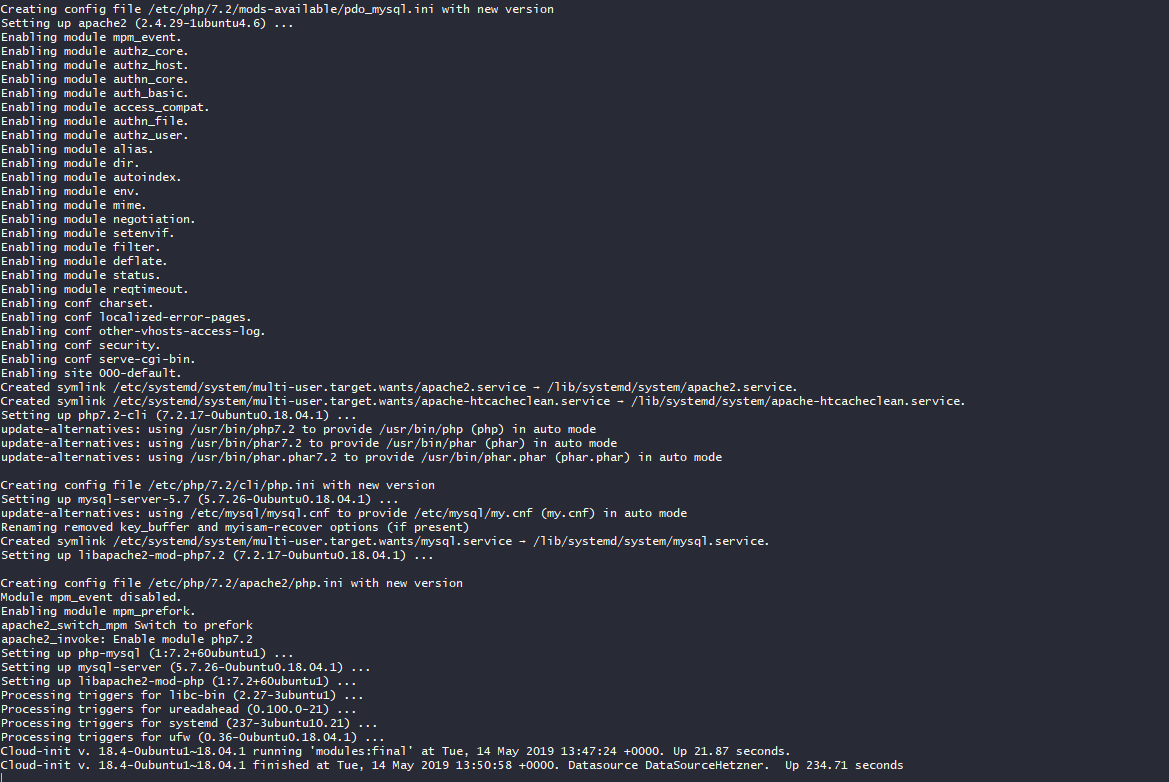
\includegraphics[width=0.45\textwidth]{img/cloudoutput.png} }}%
    \qquad
    {{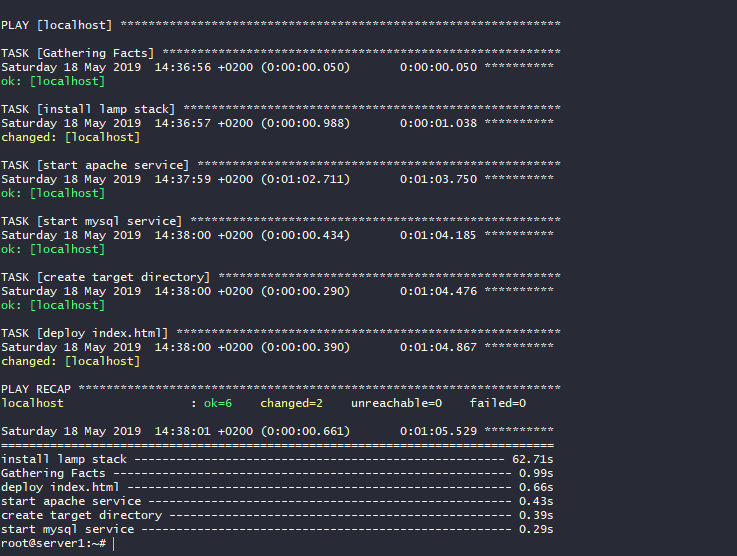
\includegraphics[width=0.45\textwidth]{img/ansibleoutput.png} }}%
    \caption{Cloud-init en Ansible outputs.}%
    \label{fig:outputs}%
\end{figure}

\section{Vergelijking met verwachte resultaten}
De verwachtingen zijn toch gedeeltelijke anders met de uiteindelijke resultaten/conclusies. In het voorstel werd er verwacht dat elke omgeving een ander oplossing ging hebben. Ook werd er verwacht dat de taken van Ansible en cloud-init gingen variëren van server tot server.

Dit is niet helemaal lijn met het effectieve resultaat. Er werd verwacht dat elke omgeving zijn eigen verhaal ging hebben en dat is toch niet gebeurt. Er kwam altijd één constante boven water. Cloud-init is goed voor de basis maar als er geavanceerder wilt gegaan worden is Ansible duidelijk beter. 

Uiteindelijk werd er verwacht dat cloud-init meer functionaliteiten ging hebben dat dat het uiteindelijk heeft. Er werd wel verwacht da Ansible ruimer ging zijn van mogelijkheden, aangezien dit veel populairder is. Maar er werd niet verwacht dat cloud-init er zoveel minder ging hebben.


\section{Verdere uitbreiding?}
Het onderzoek kan worden uitgebreid. Een restrictie die dit onderzoek had, is dat er maar één cloud omgeving kon worden gewerkt. Het zou interessant om te bekijken of er in andere omgevingen hetzelfde resultaat zou zijn of misschien iets helemaal anders. Ook de aanroeping van het cloud-init script en Ansible playbook kan op een andere manier. Door dit aan te aanroepen via een andere server, en deze scripts daardoor dus niet uit te voeren op de localhost. 

De uiteindelijke vragen die na dit onderzoek kunnen worden gesteld zijn.:
\begin{itemize}
    \item Hebben andere cloud-providers hetzelfde resultaat? 
    \item Heeft een andere aanroeping van de scripts een effect op het resultaat?
\end{itemize}

